%% LaTeX2e class for student theses
%% sections/content.tex
%%
%% Karlsruhe University of Applied Sciences
%% Faculty of  Computer Science and Business Information Systems
%% Distributed Systems (vsys)
%%
%% Prof. Dr. Christian Zirpins
%% christian.zirpins@hs-karlsruhe.de
%%
%%
%% Version 0.2, 2017-11-15
%%
%% --------------------------------------------------------
%% | Derived from sdqthesis by Erik Burger burger@kit.edu |
%% --------------------------------------------------------

\chapter{Implementierung eines ActivityPub Prototyps}
In diesem Kapitel wird die konkrete Implementierung des Prototypen, welcher für das Unternehmen angefertigt wurde in der die Abschlussarbeit bearbeitet wird, erläutert. Zu Beginn wird die Abfragesprache \glqq GraphQL\grqq~sowie die genutzte Graph-Datenbank des Projekts vorgestellt, für welches die Implementierung angefertigt wird. Danach gibt ein Klassendiagramm der Service- und Datenschicht Aufschluss über die in diesen Klassen enthaltene Funktionalität welche darauf folgend genauer beschrieben wird. Anschließend werden anhand der Verzeichnisstruktur die Controller-Schicht, sowie die Werkzeug und Sicherheitsfunktionalitäten beschrieben. Es werden zusätzlich auch die genutzten Testwerkzeuge und zwei Vorgehensweisen der Softwareentwicklung kurz erläutert. Unterkapitel \ref{sec:server-zu-server-prot} gibt Aufschluss über die implementierte Funktionalität des ActivityPub Standards. Zuletzt wird ein genauerer Blick auf die Signierung sowie Verifikation geworfen.\\

Im Jahre 2015 wurde eine Abfragesprache und Laufzeitumgebung namens GraphQL veröffentlicht, welche schon seit 2012 von mobilen Facebook Applikationen verwendet wird und somit auch von diesem Unternehmen entwickelt wurde. GraphQL nutzt zum Beschreiben der Daten ein Typsystem. Das Datenschema wird über eine Schema-Datei angegeben\cite{graphql}. Der Vorteil gegenüber einer HTTP- oder REST-\gls{api} liegt in der Nutzung eines einzelnen Endpunktes und einem Typsystem. Damit entfallen viele HTTP Anfragen, da sich mehrere Datensätze verschiedenen Typs bequem über eine Anfrage anfragen lassen. Möchte man beispielsweise für eine Statistik alle Nutzer sowie Artikel erhalten, kann dies in einer einzigen HTTP Anfrage an die GraphQL \gls{api} erledigt werden. Bei einer REST-\gls{api} müssen im schlimmsten Falle zuerst alle Identifikatoren abgerufen werden um mit diesen die eigentlichen Nutzer und Artikel abzufragen.\\

Die GraphQL-Schnittstelle kann verschiedene relationale-, nicht relationale sowie Graph-Datenbanken nutzen. Das Projekt verwendet eine Graph-Datenbank mit dem Namen \glqq Neo4j\grqq. Im Allgemeinen besteht ein Graph aus Knoten und Kanten wobei ersteres z. B. einen Nutzer mit verschieden Eigenschaften wie Passwort und Email darstellt sowie eine Kante Relationen zwischen Knoten repräsentiert wie z. B. Nutzer A ist befreundet mit Nutzer B. Speziell für das Repräsentieren und Abfragen von Relationen ist eine Graph-Datenbank bestens geeignet. Außerdem bleibt die Performanz der Abfragen konstant auch wenn die in der Datenbank enthaltene Menge an Daten steigt\cite{neo4j}.\\
\begin{figure}[h]
	\begin{minipage}{\textwidth}
		\centering
		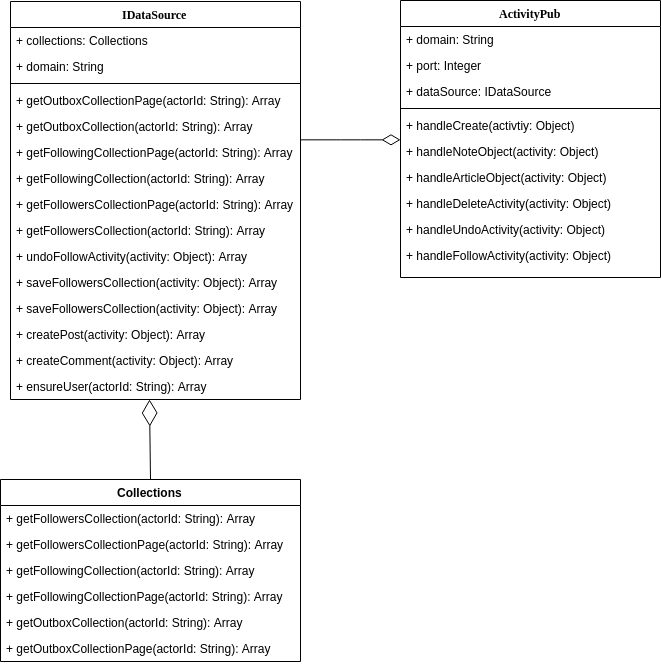
\includegraphics[scale=0.55]{figures/klassendiagramm-activitypub.png}
		\label{klassendiagramm-activitypub}
		\caption{Hauptkomponenten des förderierten Servers}
	\end{minipage}
\end{figure}
\newpage
Die Abbildung auf der nächsten Seite zeigt ein Klassendiagramm mit zwei Hauptkomponenten des Frameworks; Dies sind die ActivityPub und IDataSource Klassen. Dabei enthält die Collections Klasse das Interface, sowie das Interface die ActivityPub Klasse.\\

%% Collections Klasse grob
Die \glqq Collections\grqq~Klasse ist eine Fassaden Klasse und enthält Methoden die auf das IDataSource Interface zugreifen um folgende Sammlungen zu erhalten:
\begin{itemize}
	\item Followers Collection
	\item Following Collection
	\item Outbox Collection
\end{itemize} 
Sie dient ausschließlich dem Codeverständnis für Entwickler.\\

%% ActivityPub Klasse grob
Bei der ActivityPub Klasse handelt es sich um die Hauptklasse der Implementierung. Die entsprechenden Anfrage-Handler der Controller-Schicht wandeln die Anfrage in einen Service Aufruf um. Diese Klasse enthält nicht nur Methoden zum Verarbeiten eingehender Anfragen, sonder auch Funktionalität zum Senden von Aktivitäten.

%% NitroDataSource Klasse grob
Für eine Integration in verschiedenste Applikationen wurde das \textit{IDataSource} Interface, welches die Datenschicht repräsentiert, erstellt. Durch die Implementierung dieses Interfaces können Aktivitäten ActivityPub konform empfangen werden. Das senden wiederum muss jedes Backend selbst implementieren. Dafür stehen in der ActivityPub Klasse Methoden zum senden von Aktivitäten bereit. Durch importieren der ActivityPub Klasse erhält man eine Instanz, worüber die Methoden verfügbar sind. Zum senden werden die Daten in eine Aktivität verpackt, was über die Nutzung einer \gls{as2} Bibliothek geschehen kann oder durch Erstellung mit Objekt Literalen. Bei letzterer Variante muss sich zusätzlich um Kontexte und weiteres gekümmert werden.\\

Ein Austausch der Datenquelle ist durch die Nutzung von Datenbanken oder \glq{api}'s im Interface möglich. Es kann eine relationale oder auch nicht-relationale Datenbank, wie z. B. MySQL oder MongoDB, genutzt werden. Bei der Prototyp Implementierung in dieser Abschlussarbeit wird eine GraphQL Schnittstelle angesprochen.\\

\begingroup
	\fontsize{18pt}{12pt}\selectfont
	\textbf{Verzeichnisstruktur}
	\vspace{4pt}
\endgroup\\
\todo{Mehr sections benutzen}
\todo{subsection mit * benutzen}
\todo{Nicht sofort Bild, erst einleitender Text}
\begin{figure}[H]
	\centering
	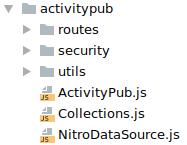
\includegraphics[width=5.5cm]{figures/activitypub-directory-structur.png}
	\caption{Ordnerstruktur des Prototypen}
	\label{fig:directory-structur}
\end{figure}
%% Controller Schicht + Ordner Funktionalität
Die Abbildung auf der letzten Seite zeigt die Verzeichnisstruktur des Frameworks. Der \glqq utils\grqq~Ordner beinhaltet verschiedene Dateien welche Funktionen mit dem Namen entsprechender Funktionalität exportieren um dies zu bewerkstelligen. In der Datei \textit{collection.js} sind Funktionen zum erstellen und senden von Sammlungen zu finden. Die Datei \textit{actor.js} beherbergt Funktionen zum Erstellen von Aktoren Objekt und WebFinger Datensatz. Funktionalität zum Erstellen, Beantworten und Validieren von Aktivitäten befindet sich in der \textit{activity.js} Datei. Jegliche weiteren Hilfsfunktionen sind in der \textit{index.js} Datei. Die zuletzt genannte Datei exportiert insgesamt 6 Funktionen. Zwei davon Erstellen Objekte (Note und Article) durch das einfügen von Werten in ein Objektliteral. Als Parameter wird den Funktionen jeweils eine activity- sowie objectId, der Inhalt, Name des Absenders sowie das Veröffentlichungsdatum übergeben. Eine weitere ist mit dem Namen des gewünschten Aktors parametrisiert für welchen der Identifikator erhalten werden soll. Des weiteren sind zwei Funktionen zum Senden von \textit{Accept} und \textit{Reject} Aktivitäten enthalten welche beide jeweils das akzeptierte oder abgelehnte Objekt, den Namen des Empfängers, sowie die Domain und \gls{url} an welche die Anfrage gesendet wird, als Parameter übergeben bekommen. Die letzte exportierte Funktion gibt einen Wahrheitswert zurück, welcher angibt ob das Notiz oder Artikel Objekt an die Öffentlichkeit gesendet wird.\\
\todo{utils Funktionen vlt. genauer beschreiben}
\begin{figure}[H]
	\centering
	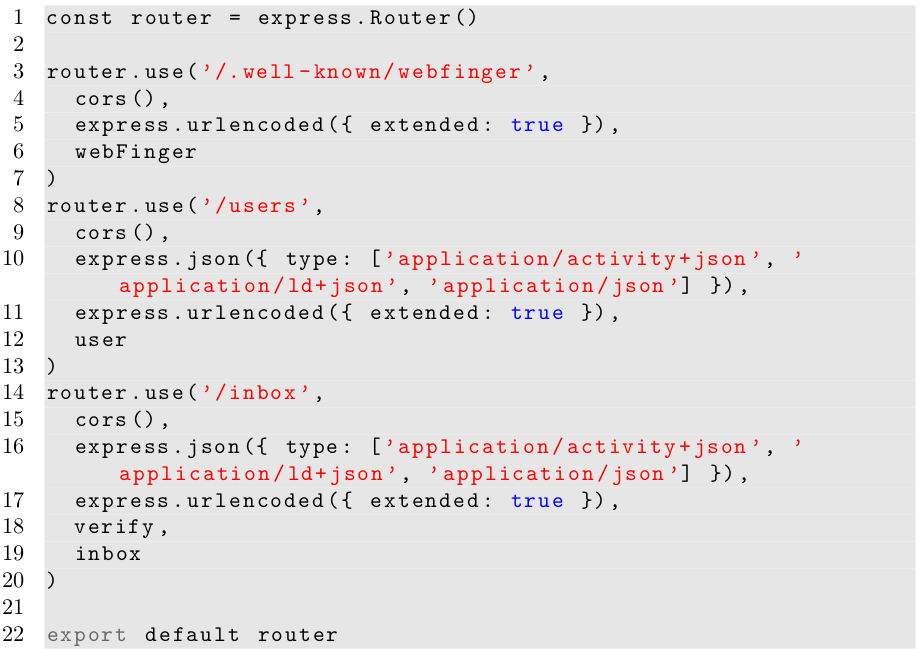
\includegraphics[width=15cm]{figures/router-index.png}
	\caption{Wie die einzelnen Teile zusammengefügt werden}
	\label{fig:router-index}
\end{figure}
Alle Controller befinden sich im  \textit{router} Ordner. Jede Datei beinhaltet einen Express Router, welche alle in der \textit{index.js} Datei zu einem einzigen zusammengefasst werden (siehe Abb. \ref{fig:router-index}). Dabei nutzt jeder Router zusätzlich die Express \gls{cors} Middleware um entsprechend die HTTP Verben \textit{Post}, \textit{GET} oder beide für den Zugriff von anderen Domains freizugeben. Außerdem wird bei allen Nutzer betreffenden Routen, sowie beim geteilten Nachrichteneingang ein Parser genutzt um Anfrage Inhalte mit den drei gegebenen Inhaltstypen (\textit{application/json, application/ld+json, application/activity+json}) in Objekte umzuwandeln und eine weitere Middleware für das Parsen der \gls{url} Parameter. Bei eingehenden Nachrichten, welche Daten verändern wird des weiteren ein Router benutzt um die HTTP Signaturen zu verifizieren.\\

Bei ausgehenden Anfragen wir Funktionalität benötigt um Signaturen zu erstellen welche im \textit{security} Ordner bereitgestellt wird. Nicht nur zur Signierung ausgehender, sonder auch zum Verifizieren eingehender Anfragen ist eine Funktion vorhanden. Signiert sowie Verifiziert werden können die Anfragen mit verschiedenen bekannten Hashfunktionen, wie z.B. \textit{SHA-256}, \textit{MD5} oder \textit{SHA-512}, in Kombination mit einem Schlüsselpaar eines öffentlichen Schlüssel Verfahrens. Genutzt wird dazu die in Node.js enthaltene \textit{crypto} Bibliothek.\\

Die \textit{index} Datei im \textit{security} Ordner exportiert drei Funktionen und ein Array mit unterstützten Hashfunktionen. Wird ein \gls{rsa} Schlüsselpaar benötigt kann dieses mit der \textit{generateRsaKeyPair} Funktion generiert werden. Diese bekommt als Parameter ein Options Objekt mit \textit{passphrase} Eigenschaft übergeben; Es genügt auch ein parameterloser Aufruf wobei die Umgebungsvariable \glqq PRIVATE\_KEY\_PASSPHRASE\grqq~ausgelesen wird.\\

Zur Erstellung einer HTTP Signatur wird die \textit{createSignature} Funktion verwendet. Wie die vorherige bekommt auch diese als Parameter ein \textit{options} Objekt übergeben. Dieses benötigt einen privaten Schlüssel welcher zur Signierung verwendet wird, sowie eine \textit{keyId} (Referenz auf den öffentlichen Schlüssel) und \textit{url} als Eigenschaften. Mit der \textit{headers} Eigenschaft kann optional angegeben werden, welche Kopfzeilen bei der Signierung Verwendung finden. Die Datums Kopfzeile wird standardmäßig genutzt und muss somit nicht angegeben werden. Weitere optionale Eigenschaften sind \textit{algorithm} und \textit{passphrase}, wobei letzteres wie zuvor aus der Umgebung ausgelesen wird. Eine Hashfunktion kann unter den im exportierten Array enthaltenen gewählt werden. Beim Aufruf der \textit{createSignature} Funktion wird zuerst der verwendete Algorithmus validiert und anschließend unter Verwendung des privaten Schlüssels und einer Passphrase, sowie einer zuvor konstruierten Zeichenkette die Signatur in der Base64\footnote{Base64 ist ein Verfahren zu Kodierung von 8-Bit Binärdaten in ASCII-Zeichen} Kodierung erstellt.\\

Die Parameter der dritten exportierten Funktion, \textit{verifySignature}, sind einmal der Endpunkt mit, falls vorhanden, Suchanfrage an welchen die HTTP Anfrage gesendet wurde und zweitens die Kopfzeilen. Aus den Kopfzeilen werden beim Aufruf der Funktion die Signatur genommen und aus dieser alle Werte extrahiert. Danach wird die Zeichenkette welche neben privatem Schlüssel und Passphrase zum Signieren verwendet wurde rekonstruiert. Über die \textit{keyId} wird der öffentliche Schlüssel angefragt und mit diesem, der Signatur, der Zeichenfolge und dem verwendeten Algorithmus als Parameter, die Funktion zum Erstellen der Komponente zur Verifikation und dem eigentlichen verifizieren aufgerufen.\\

\begingroup
	\fontsize{18pt}{12pt}\selectfont
	\textbf{Funktionalität und Änderungen}
	\vspace{4pt}
\endgroup\\
%% NitroDataSource Klasse
Das IDataSource Interface enthält Methoden zum beziehen, sowie speichern von Sammlungen. Als Parameter bekommen die Methoden zum beziehen von Sammlungen die \glqq actorId\grqq~übergeben. Aus dieser kann der Nutzername extrahiert und so die entsprechenden Daten verarbeitet werden, welche unter Zuhilfenahme von Hilfsfunktionen aus dem Werkzeug Ordner zu Sammlungen konvertiert werden. Die Methoden zum speichern bekommen eine Sammlung übergeben welche zuvor mit den Hilfsfunktionen erstellt wurden. Optional kann mit einer Flagge angeben werden, ob nur das neuste Element gespeichert werden soll.\\

Weiter enthält das IDataSource Interface Methoden zum Erstellen und Löschen von \glqq Post's\grqq~, Kommentaren sowie \glqq Shout's\grqq\footnote{Ein \glqq Shout\grqq~ist mit einem \glqq Like\grqq~in anderen Netzwerken zu vergleichen.} und zusätzlich zum Updaten von \glqq Post's\grqq. Alle in diesem Absatz genannten Methoden bekommen eine Aktivität als Parameter übergeben. Diese wird über das Umwandeln in eine GraphQL Anfrage und ausführen dieser in einer dem Hauptsystem entsprechenden Repräsentation gespeichert.\\

Um zu wissen an welche Server eine ausgehende Aktivität gesendet werden soll ist auch Funktionalität zum beziehen und hinzufügen von geteilten Nachrichteneingängen vorhanden. Bei Eingehende Anfragen, welche bei der Verarbeitung das Aktoren-Objekt eines Nutzers beziehen, wird geprüft ob der geteilte Nachrichteneingang bereits hinzugefügt wurde. Ist das nicht der Fall wird dieser den bekannten hinzugefügt. So entsteht ein \glqq bekanntes Netzwerk\grqq.\\

Zum sicherstellen ob ein Nutzer bereits existiert sowie zum rückgängig machen eines vorherigen folgens wird des weiteren Funktionalität bereitgestellt. Für jeden gesichteten Nutzer wird eine der Implementierung entsprechende Repräsentation im Netzwerk angelegt mit einem zufällig generierten Passwort. Dadurch müssen keine weiteren Typen dem GraphQL Schema hinzugefügt und außerdem keine neuen Relationen angelegt werden.\\

Ein paar Änderungen sind dennoch nötig. Der Nutzertyp wird um drei Eigenschaften erweitert: Erstens der \glqq actorId\grqq~, zweitens um einen privaten und drittens einen öffentlichen Schlüssel. Außerdem muss für alle Modelle, im GraphQL Schema Typen genannt, eine Aktivitäten- und Objektidentifikator Eigenschaft angelegt werden. Dadurch wird die vollständige rekonstruiert entsprechender \gls{as2} Objekte und Aktivitäten sichergestellt.\\

\begingroup
	\fontsize{18pt}{12pt}\selectfont
	\textbf{Testwerkzeuge}
	\vspace{4pt}
\endgroup\\
Getestet wird die Implementierung mit dem Cucumber Test-Framework, welches ein Werkzeug zum ausüben von \gls{bdd} ist. Es wurden Akzeptanz Tests erstellt um zu prüfen ob der Service ActivityPub konform ist. Die Tests selbst werden im Rahmen von Cucumber als sogenannte \glqq Feature\grqq's bezeichnet und haben die Dateiendung \glqq .feature\grqq. Geschrieben sind die Tests in der Gherkin Sprache welche eine Sammlung von Syntax ist um diese auf entsprechende Aktionen, sogenannte \glqq Steps\grqq~abzubilden. Nicht nur einzelne \glqq Step\grqq~Definitionen sonder auch Welt Dateien können genutzt werden um einen Ort für wiederverwendbare Funktionalität zu haben und einen Testzustand einzuführen. Es wurden bei der Gherkin Syntax extra leicht verständliche Schlüsselworte gewählt um die Tests auch für Benutzer, Produktbesitzer und weitere lesbar zu halten. Somit muss nur die Gherkin Sprache bekannt sein um die Features schreiben zu können. Das Verständnis beim lesen ergibt sich aus der Verwendung natürlicher Sprachkonstrukte als Schlüsselwörter. Die \glqq Step\grqq~Definitionen zu implementieren setzt allerdings, im Gegensatz zum schreiben von \glqq Features\grqq~Dateien, Programmierkenntnisse voraus.\\

\begingroup
	\fontsize{18pt}{12pt}\selectfont
	\textbf{Vorgehensweisen in der Softwareentwicklung}
	\vspace{4pt}
\endgroup\\
Unter \gls{tdd} versteht man eine Vorgehensweise beim Entwickeln von Software. Dabei werden zuerst fehlschlagende Tests geschrieben, um diese im zweiten Schritt durch eine Implementierung der Komponenten zur erfolgreichen Ausführung zu bringen. Im dritten Schritt werden die Tests angepasst und der Zyklus wiederholt sich.\\

Bei der Softwareentwicklung mit dem \gls{bdd} Ansatz wird im Grunde genommen Wert auf eine hohe Kommunikation zwischen allen beteiligten im Entwicklungsprozess gelegt. Werkzeuge wie Cucumber fördern dabei die Lesbarkeit von Softwaretests und somit auch die Kommunikation zwischen Programmierern und dem Rest des Teams. Zudem ist es für Neueinsteiger leichter einen Überblick über die Funktionalität des Systems zu bekommen\footnote{Vlg. Cucumber Gemeinschaft, Absatz 1}.\\
 
\section{Server-zu-Server Protokoll}
\label{sec:server-zu-server-prot}
Es wird eine Teilmenge der \gls{as2} Objekte und Aktivitäten implementiert, die angepasst ist auf die Anforderungen des Unternehmens in welcher diese Arbeit angefertigt wird. Dabei handelt es sich um folgende Aktivitäten: \textit{Create}, \textit{Update}, \textit{Delete}, \textit{Follow}, \textit{Undo}, \textit{Accept}, \textit{Reject}, \textit{Like}, \textit{Dislike}. Als Objekt Eigenschaft der Aktivitäten werden folgende Typen implementiert: \textit{Note}, \textit{Article}.\\

Die ersten drei Aktivitäten werden zum Manipulieren von Objekten wie z. B. einem Artikel benötigt. \textit{Follow} und \textit{Undo} sind zum folgen eines Nutzers so wie zum rückgängig machen verschiedener Aktivitäten. Wenn einem Nutzer gefolgt wurde, wird eine \textit{Accept} Aktivität an die \textit{Inbox} des Folgenden gesendet mit einer \textit{Follow} Aktivität als Objekt. Im Falle eines Fehlers wird die Anfrage mit einer \textit{Reject} Aktivität beantwortet.\\

Der Funktionsumfang des förderierten Servers beschränkt sich auf den folgenden:
\begin{itemize}
	\item Empfangen von \textit{\textbf{Article}} und \textit{\textbf{Note}} Objekten am Geteilten Nachrichteneingang (sharedInbox)
	\item Empfangen von \textit{\textbf{Like}} und \textit{\textbf{Follow}} Aktivitäten am Geteilten Nachrichteneingang
	\item Empfangen von \textit{\textbf{Undo}} und \textit{\textbf{Delete}} Aktivitäten für \textit{\textbf{Articles}} und \textit{\textbf{Notes}} am Geteilten Nachrichteneingang 
	\item Bereitstellen eines \textit{\textbf{Webfinger}} und \textit{\textbf{Aktoren}} Objektes
	\item Bereitstellen der \textit{\textbf{Followers}}, \textit{\textbf{Following}} und \textit{\textbf{Outbox}} Sammlungen
\end{itemize}

Artikel und Notizen werden bei der in dieser Arbeit angefertigten Implementierung gleich behandelt. Beim empfangen einer Create Aktivität, die eine Notiz oder Artikel als Objekt Attribut hat, wird der Artikel über die IDataSource Implementierung erstellt und entsprechende Metadaten zum rekonstruieren der ID's gespeichert. Somit können empfangene \glqq Posts\grqq, welche an die Öffentlichkeit gerichtet sind, im Netzwerk angezeigt werden. Die Logik zum Empfangen von \glqq Posts\grqq~die an einzelne Nutzer gerichtet sind ist noch nicht vorhanden.\\

\begingroup
	\fontsize{18pt}{12pt}\selectfont
	\textbf{Signierung und Verifikation}
	\vspace{4pt}
\endgroup\\
Eingehende HTTP POST Anfragen werden auf eine vorhandene Signatur Kopfzeile geprüft. Wird diese nicht gefunden, wird die Anfrage verworfen. Ist sie vorhanden, wird die Signatur geprüft indem das Aktoren Objekt über die zugehörige \textit{keyId} angefragt wird und die Signatur gegen den öffentlichen Schlüssel geprüft wird. Dies stellt sicher, das die Inhalte der Nachricht beim Transport nicht verändert wurde und zudem das die Aktivität von dem Nutzer stammt, der den passenden privaten Schlüssel besitzt. Eine Signatur bei der Übertragung von Servern untereinander wird demnach verwendet um die Authentizität der Daten überprüfen zu können.\\

Für die Nutzung eines Schlüsselpaars pro Aktor spricht, dass es für potentielle Angreifer schwieriger wird die Schlüssel zu erhalten. Bei der Nutzung eines einzigen Server Schlüsselpaars zur Signierung und Verifikation, reicht es dieses zu entwenden. Es sei angemerkt das die privaten Schlüssel mit einer Einweg Hashfunktion, in Verbindung mit einem Passwort, verschlüsselt werden und dieses Passwort somit zusätzlich entwendet werden muss.\\

Bei dieser Implementierung gibt es keine Server-zu-Server Interaktionen die nicht vom Nutzer initiiert wurden, abgesehen von der Anfrage nach Aktoren Objekten oder WebFinger Deskriptoren welche auch Nutzer initiiert sind, allerdings von Nutzern anderer Instanzen. Somit ist die Generierung eines weiteren Schlüsselpaars für den Server nicht notwendig da die Inhalte mit den entsprechenden privaten Schlüsseln der Autoren signiert werden. Darüber wird festgestellt ob der Server von dem die Anfrage kam, über den privaten Schlüssel verfügt mit welcher die Signatur erstellt wurde.